
\chapter{Methods}

\label{Methods} 

This chapter describes in detail the methods for whatever activities were necessary for your project – e.g., data gathering, data analysis, requirements analysis, design, implementation, testing/evaluation, etc. Your choice of methods should be discussed and justified in view of the project objectives, and with reference to the pertinent literature. Report not only what methods you applied in generic terms, but what you actually did: sufficient information about dates and details for your reader to understand how you ran your project, rather than just how one could run any similar project.  

Report in this chapter what you did, not what you produced or found as a 
result (which goes under Results).  
  
Note: only use the word ‘methodology’ if you know what it means!  

% LC - 14 pages

\subsection{Digital Images}
Digital images are stored as a square multidimensional matrix. A 100x100 colour images (with values from Red, Green and Blue) is represented as a matrix of dimensions $n x m x c$, where n is the width, m is the height and c is the depth (number of colour channels of the image. Black and white images have c = 1, where the pixel value is either on or off (TBC). Greyscale images also have one channel.

\subsection{Data pre-processing}
Prior to presenting pixel colour channel values to the network, a number of pre-processing steps have become standard with neural network classifiers and regressors applied to computer vision.


Explain:  
\begin{itemize}
    \item Convolution
    \item pre-processing
    \item Kernel/filter size
    \item Stride
    \item padding
    \item activation function
    \item Loss function
    \item optimisers
    \item Back-propagation
    % on this topic, a lot to cite, from Paul Werbos' PhD thesis "Beyond Regression: New Tools for Prediction and Analysis in the Behavioural Sciences, through Rummelhart et al. and LeCunn et al.
\end{itemize}

Maybe cite goodfellow once and do a joblot on items.  

Our NVIDIA architecture is very similar to the one proposed by Bojarski et al. 2016. Our alternative AlexNet, GoogleLeNet, VGGNet and ResNet however have much fewer parameters. This is due to the "degradation" problem, where the number of parameters is too large for the dataset, and the network fails to converge.

\section{Datasets}
What datasets we used and what data was gathered

% on converting GPS and IMU measurements to steering angles, see
% http://www.robesafe.uah.es/personal/roberto.arroyo/docs/Almazan13iv.pdf
% We might use a similar technique, time allowing

\subsection{Data Augmentation}
Describe was additional transformations was performed to enlarge dataset - maybe a discussion that more data is good? With references.

Found this article:
% https://lmb.informatik.uni-freiburg.de/Publications/2015/FDB15/image_orientation.pdf
Would some good suggestions:  
Augmentation. To prevent overfitting, we perform image augmentation, i.e., we
apply random transformations to input samples during network training on the
fly. We use translations (up to 5\% of the image width), brightness adjustment
% in the range [−0.2, 0.2], gamma adjustment with \\gamma \\memberof [−0.5, 0.1] and Gaussian
pixel noise with a standard deviation in the range [0, 0.02].
  
Paper is referred to by this discussion: 
% https://stats.stackexchange.com/questions/335836/cnn-architectures-for-regression
A somewhat more succinct definition of the procedure:  
% https://stats.stackexchange.com/questions/456126/could-resnet-curve-be-used-for-a-regression-problem-e-g-housing-price-predicti
Just to make it clear, a regression problem is one whose target is continuous and not discrete. In this sense you can make any Neural Network that is primarily used for classification a regressor, with minimal changes. Namely it needs to end with 1 neuron, no activation function and a proper loss function (e.g. mean squared error). For example, object detection is in its core a regression problem because you are trying to predict coordinates. Any ResNet could be used for these problems



\section{Deep Convolutional Neural Network Models}

Description of different network architectures used, noting what modifications were required.  

\textbf{Discussion on the number of parameters required given size of dataset.}  
We also need a discussion on deep regression models as suggested by \cite{lathuilire2018comprehensive}. This is the main difference between the NVIDIA and additional models, the NVIDIA model is a regression model while the models we compare and contrast with NVIDIA are classification models built specifically for the ILSVC  competitiion.

\subsection{ResNet}

Discuss the concept of "residuals". ResNet makes use of skip-connections (spelling), these "network architecture
designs (e.g., skip connections) produce loss functions that train easier", producing smoother loss surfaces (\cite{li2017visualizing})  
The "Degradation problem itself stems from the fact that it is easier to learn 0 than to learn 1"   https://www.youtube.com/watch?v=jio04YvgraU
"if an identity mapping were optimal, it would be easier to push the residual to zero than to fit an identity mapping by a stack of nonlinear layers" \cite{he2015deep}.  
Explain what variation A, B or C we will be using (zero padding, weights * x, etc.  
"Essemble" of ResNets was used.  
18 layers seems to be a threshold, beyond that, training becomes difficult. Skip connections make deeper networks, i.e. networks with more layers, easier to train compared to networks without skip connections.  
Another wording, deeper neural networks (i.e. layer count equal or greater than 20) become increasingly difficult to train, generating poorer accuracy than deep networks with less than 20 layers. This is known as "degradation problem" (citation needed). Skip connections make deeper architectures easier to train, by smoothing the loss function.

\subsection{GoogleLeNet}

This network (\cite{szegedy2014going}) was the winning entry in the ILSVCC 2014 Classification Challenge. It uses the LeNet-5 (\cite{Lecun98gradient-basedlearning}) model as a starting point, following the now traditional design of ConvNets with the addition of \textit{Inception} modules as introduced by \cite{lin2013network} in the \textit{Network in Network} model.

\begin{figure}[ht]
 \centering 
 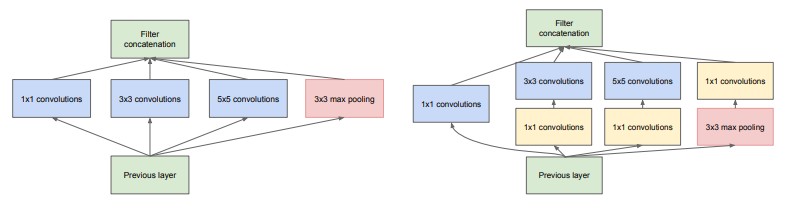
\includegraphics[width=\columnwidth]{Figures/InceptionModules.png}
 \caption{Inception naive (left) and dimension reduction model (right)}
 \label{fig:inception_modules}
\end{figure}

The designers of the GoogleLeNet architecture state that power and memory use is important to consider and aim to keep a computation budget of 1.5 billion multiply adds at inference time such that the resulting model could be used in practice at a reasonable cost.

The architecture contains 22 layers where all

\subsection{Deep Regression Models}
Explain the process of transforming these models (except NVIDIA) into regression models, maybe cite \cite{Lathuiliere_2020} or papers cited therein.

\subsection{Binning/Quantization}
Describe this approach, if we get that far, to use an alternative to regression models, whereby we may bin the outputs. This could potentially simplify the model. Also, depending on track, we could have narrower bins around zero degrees, i.e. finer control and wider bins away from zero degrees, i.e. coarser control. Or vice-versa - experimentation required.

\subsection{Training}

We might want to add that training was done on AWS GPUs following   
https://aws.amazon.com/blogs/machine-learning/train-deep-learning-models-on-gpus-using-amazon-ec2-spot-instances/  


\section{Evalutation}
This section discussed the evaluation benchmarks, here we discuss the evaluation environment (Unity 3D game engine) and how it was used to both generate data and evaluate the models.

%% Udacity
%% see https://arxiv.org/pdf/1912.05440.pdf
%% for discussion on using rmse as error metric


